
\documentclass{standalone}

\usepackage{amsmath} 
\usepackage{tikz}

\begin{document}
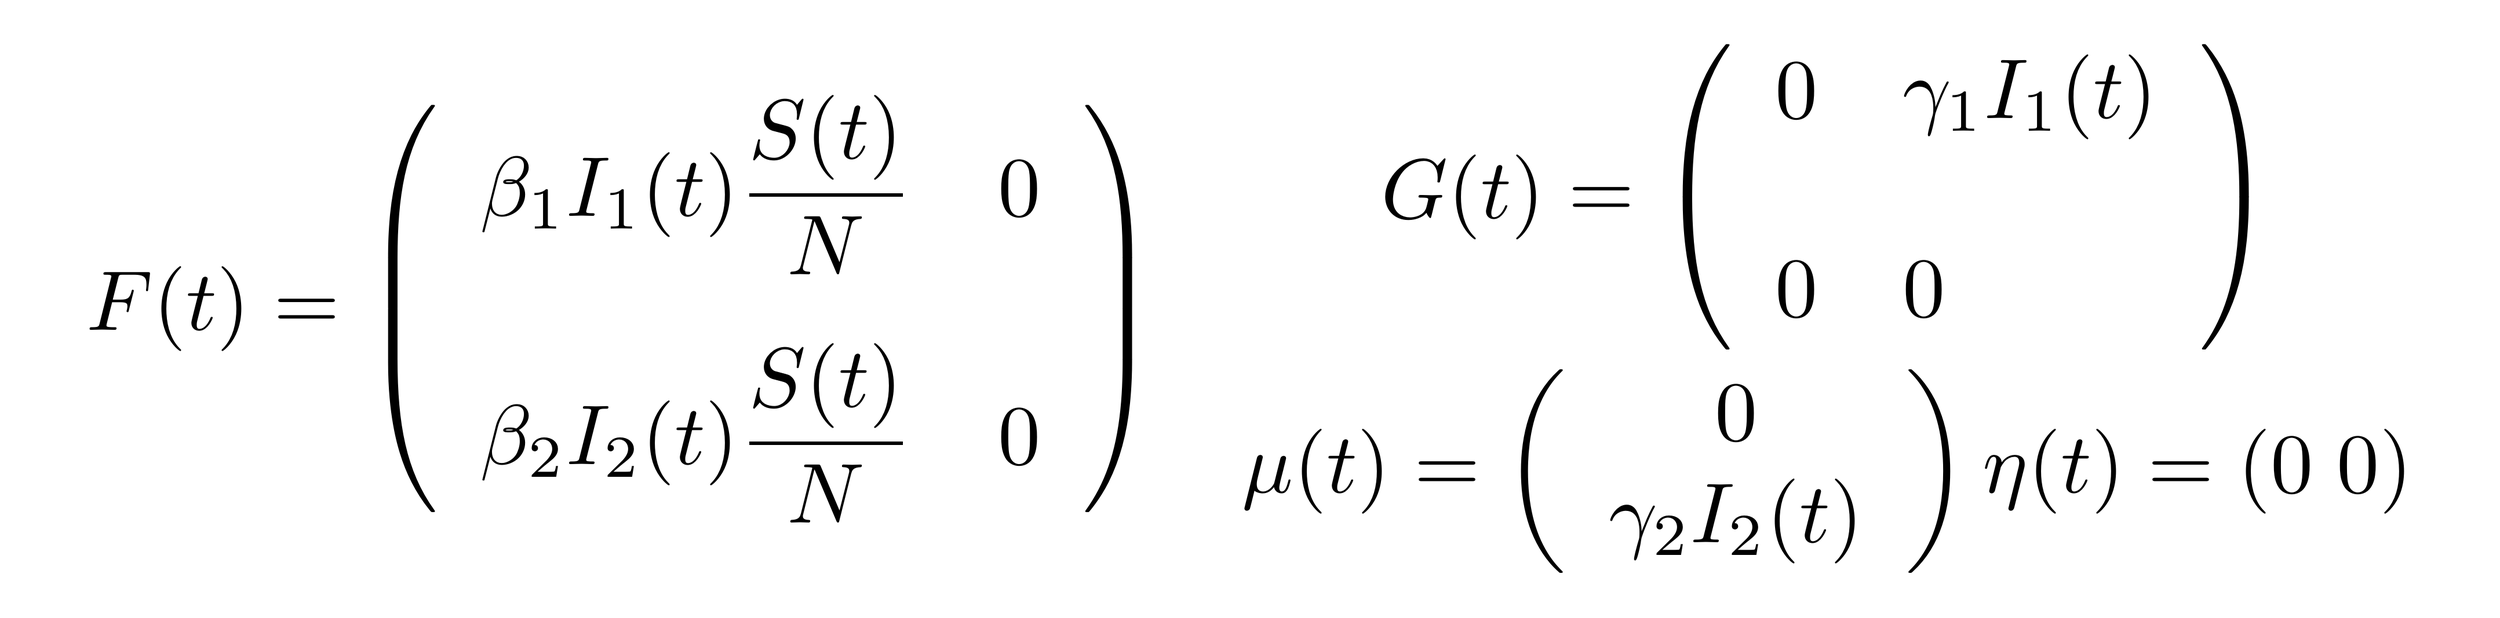
\begin{tikzpicture}
\node[scale=5.3]  {
$
\begin{array}{c}
F(t)  = \left(  \begin{array}{ll}
\beta_1 I_1(t) \dfrac{S(t)}{N} & 0 \\[4mm]
\beta_2 I_2(t) \dfrac{S(t)}{N} & 0
\end{array}
\right)
\end{array}
% \quad
\begin{array}{c}
G(t) =  \left(  \begin{array}{ll}
0 & \gamma_1 I_1(t)  \\[4mm]
0 & 0
\end{array}
\right)
\\ [0.5cm]
\mu(t) = \left( \begin{array}{c}
0 \\ \gamma_2 I_2(t)
\end{array} \right)
\eta(t) = (0 \; 0)
%\eta(t) = \left( \begin{array}{c}
%0 \\ 0
%\end{array} \right)
\end{array}
$
};
\end{tikzpicture}
\end{document}